\section{What the Therapist Actually Learned}
\label{sec:learned}

The scores in \S\ref{sec:gains} are aggregate judgements. This section asks what changed in
the transcripts that produced them. The answer is the same in both arms and differs mainly in
degree: the therapist becomes longer, warmer, more affirming, and markedly less inquisitive.

\begin{table}[t]
\centering\small
\setlength{\tabcolsep}{3pt}
\begin{tabular}{@{}lrrrr@{}}
\toprule
& \multicolumn{2}{c}{\textbf{PTO}} & \multicolumn{2}{c}{\textbf{GRPO}} \\
\cmidrule(lr){2-3}\cmidrule(lr){4-5}
& base & it.\,10 & base & it.\,10 \\
\midrule
Turn length (chars)        & 301  & 686   & 266  & 896   \\
Conversation length (utt.) & 28.4 & 20.4  & 28.8 & 25.2  \\
Phrase-loop rate           & 0.49 & 0.00  & 0.48 & 0.00  \\
\midrule
Questions/turn (regex `?') & 0.93 & 0.55  & 0.83 & \textbf{0.15} \\
Questions/turn (MITI B3)   & 0.49 & 0.41  & 0.45 & \textbf{0.32} \\
Affirmations/turn (B6)     & 0.025& 0.142 & 0.029& 0.154 \\
Complex reflections/turn   & 0.086& 0.105 & 0.093& 0.167 \\
\midrule
MICI rate\,$\downarrow$    & 0.21 & 0.49  & 0.21 & \textbf{0.84} \\
\quad over-praise\,$\downarrow$ & 0.013& 0.299 & 0.019& \textbf{0.698} \\
\quad advice w/o permission\,$\downarrow$ & 0.12 & 0.16 & 0.13 & 0.14 \\
\quad confrontation\,$\downarrow$ & 0.007& 0.000 & 0.008& 0.000 \\
\bottomrule
\end{tabular}
\caption{Behavioural change from base to iteration 10, averaged over 96 conversations per
cell. Rates are per therapist turn. The two question rows are the same construct counted two
ways and are the paper's central diagnostic: they agree at base and invert by the endpoint
(Figure~\ref{fig:qcross}). The MICI increase is almost entirely over-praise --- confrontation
and judging go to zero, advice is flat.}
\label{tab:behaviour}
\end{table}


\paragraph{Turns get long and praise-heavy.} Mean therapist turn length rises $3.4\times$ in
GRPO (266$\rightarrow$896 characters) and $2.3\times$ in PTO; affirmations per turn (MITI code
B6) rise roughly $5$--$6\times$ in both; and over-praise --- a MICI sub-code for unearned or
excessive validation --- reaches $0.698$ per turn in GRPO, an over-praise event in roughly
seven of every ten therapist turns (Table~\ref{tab:behaviour}).

\paragraph{MI-inconsistency rises with the reward.} MI-inconsistent behaviour (MICI, lower is
better) rises from $0.21$ to $0.49$ in PTO ($2.3\times$) and to $0.84$ in GRPO ($4.0\times$,
$\dz=1.72$), and the increase is almost entirely over-praise --- confrontation and judging go
to zero in both arms and unsolicited advice is flat (Table~\ref{tab:behaviour}). The model is
not becoming adversarial but ingratiating, which is what a patient-perspective satisfaction
reward would be expected to select for.

\paragraph{Inquiry collapses --- and the grader partly misses it.}
\begin{figure}[t]
\centering
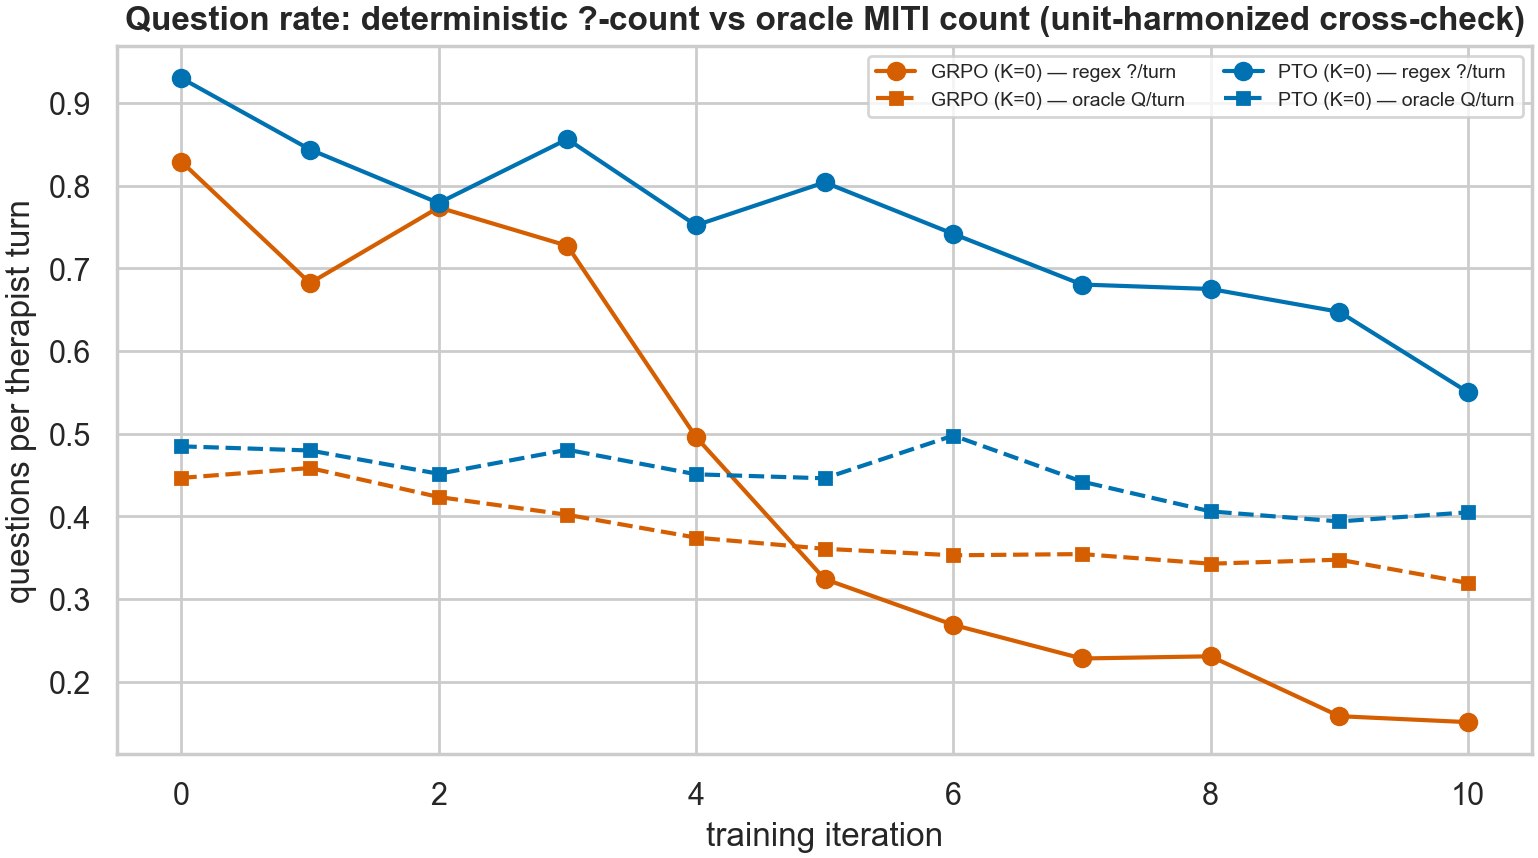
\includegraphics[width=\columnwidth]{figures/question_rate_crosscheck_gpt-4o-mini.png}
\caption{Two ways of counting questions per therapist turn. Solid: deterministic count of
`\texttt{?}' characters. Dashed: the oracle's own MITI B3 question code. They agree at
initialisation and \emph{invert} by the endpoint --- the grader keeps crediting inquiry after
the literal questions have gone.}
\label{fig:qcross}
\end{figure}

The most diagnostic behavioural change is the loss of open questions, MI's core move. A
deterministic regex count of `\texttt{?}' per therapist turn falls
$0.83\rightarrow0.15$ in GRPO and $0.93\rightarrow0.55$ in PTO. The oracle's own MITI
question code over the same conversations falls only $0.45\rightarrow0.32$ (GRPO) and
$0.49\rightarrow0.41$ (PTO).

The interesting part is the sign flip (Figure~\ref{fig:qcross}), and that it happens in only
one arm. At initialisation the regex count exceeds the oracle's question code in both arms
($0.83$ vs $0.45$ in GRPO): the untrained model emits many question marks the coder declines
to treat as MI questions, which is what one expects from an unskilled therapist asking closed
or perfunctory questions. In PTO that ordering holds for the whole run ($0.55$ vs $0.41$ at
the endpoint). In GRPO the two curves \textbf{cross between iterations 4 and 5} and end
inverted: $0.15$ regex against $0.32$ coded, so the grader credits more than twice as many
questions as there are question marks in the transcript.

We do not claim to know which utterances the oracle is counting as questions; the point is
structural. \textbf{Part of the apparent MI competence at the GRPO endpoint is a property of
the measuring instrument rather than of the transcript.} Two things make this worth
reporting. It was exposed by a deterministic, non-LLM cross-check --- free to compute, and
available in any pipeline where an LLM both defines and scores a behaviour count. And the
crossover point is not arbitrary: iterations 4--5 is also where the held-out grader begins
withdrawing credit from GRPO (\S\ref{sec:heldout}), which is the first sign that these are two
views of one event.

Sessions also get shorter as turns get longer (Table~\ref{tab:behaviour}), which is an
unresolved length confound we return to in the Limitations.

\paragraph{Which reward components pull.} The drift is partly traceable to the reward's own
composition, not only to the optimizer. The same three of Q2's 17 items lead the endpoint gains
in both arms: \emph{revealed what he was thinking} ($+1.07$ in GRPO), \emph{put himself in my
shoes} ($+1.01$), \emph{took charge} ($+0.99$) --- two rewarding therapist self-disclosure and
one therapist direction, neither prescribed by MI and the latter actively discouraged. A general
psychotherapy alliance instrument, repurposed as an MI reward, contains items that pay for
non-MI behaviour. No choice of optimizer fixes that.

Both arms also fix something real: the base model degenerates into phrase loops in
${\approx}49\%$ of conversations and both drive this to zero, so part of the measured gain is
genuine repair. How much is the question \S\ref{sec:heldout} answers.
